\documentclass[sigconf,nonacm]{acmart}
\usepackage{tikz}
\usepackage{xcolor}
\usetikzlibrary{arrows.meta,positioning}
\usepackage{tabularx,booktabs}
\settopmatter{printacmref=false,printccs=false,printfolios=true,authorsperrow=4}
\setcopyright{none}
\renewcommand\footnotetextcopyrightpermission[1]{}
\pagestyle{plain}
\title{PRISM: Background and Related Work on Privacy-Constrained Customer Churn Classification}
\author{Abhishek Majumdar}
\affiliation{\institution{University of Victoria}\city{Victoria}\country{Canada}}
\author{Dev Parsana}
\affiliation{\institution{University of Victoria}\city{Victoria}\country{Canada}}
\author{Ravi Vashi}
\affiliation{\institution{University of Victoria}\city{Victoria}\country{Canada}}
\renewcommand{\shortauthors}{Majumdar et al.}
\begin{document}
\begin{abstract}
Customer churn prediction supports retention decisions, but a useful model may need to operate with limited amount of customer information. We researched the development of churn modelling, talked about predictive and data-minimization methods, and compare their data requirements and limitations. PRISM investigates the predictive cost of restricting account attributes through predefined visibility tiers. Our contribution is a controlled comparison under different information availability, rather than a guaranteed claim of privacy. 
Our contribution is a controlled comparison
under different information availability, rather than
a guaranteed claim of privacy.
Repository: \url{https://github.com/ParsanaDev/PRISM-churn-privacy}.
\end{abstract}
\maketitle

\section{Introduction}
Customer churn is the loss of existing customers. In subscription-based services, recorded cancellations provides a baseline criteria which in-turn become labels for supervised binary classification(churn, no churn). The challenge considered by PRISM is whether useful predictions are possible when only a restricted set of account attributes is available. Prior work evaluates predictive methods and maximizing profit through retention ~\cite{mozer,neslin}; whereas data-minimization research separately examines how much input information a model needs~\cite{goldsteen}. Together, these two method motivate PRISM’s core comparison: measuring how churn-prediction performance changes as we restrict the information a model can access, using explicitly defined attribute tiers. This restriction is evaluated purely in terms of analyzing predictive cost, since account metadata is still potentially personal data; using fewer attributes does not, by itself, guarantee privacy protection or legal compliance.

\section{Historical Background}
The underlying problem arises even before computing existed. Understanding why buyers return to a seller or switch elsewhere is well explained in  Copeland's 1923 discussion of buying habits and brand preference or insistence~\cite{copeland}. By 2000, Mozer et al.~\cite{mozer} applied statistical machine learning to wireless subscriber churn using operational customer records. Subsequent work compared many predictive modelling choices to figure out which one works~\cite{neslin} . Scalable tree boosting~\cite{xgboost} expanded the available modelling tools, whereas input-minimization methods~\cite{goldsteen} shifted attention toward retaining utility with less detailed information.

\section{Hierarchy of Related Approaches}
Figure~\ref{fig:taxonomy} organizes the reviewed methods by their main function. \textit{Predictive methods} estimate churn from labelled customer records; their subcategories distinguish statistical, tree-based, and neural models. \textit{Input-minimization methods} modify the information supplied to a classifier(predictor), through feature suppression or value generalization. The two branches are independent, any restricted feature set can be paired with any classifier family. Varying both at once would confound their effects, so PRISM sets a fixed classifier and changes between different information tiers; and comparison between classifiers occurs only within a specific tier. The above hierarchy includes only methods relevant to this comparison.

\begin{figure}[t]
\centering
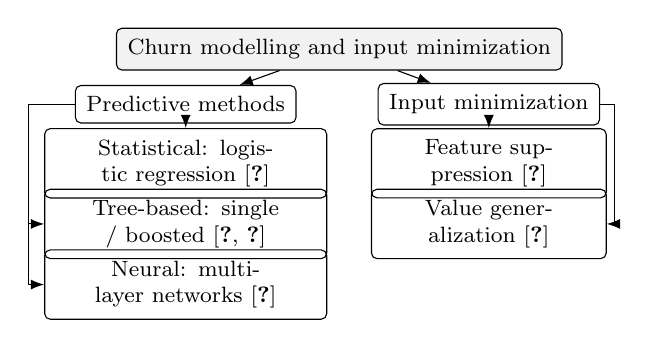
\begin{tikzpicture}[font=\footnotesize,box/.style={draw,rounded corners=2pt,align=center,inner sep=4pt},line/.style={-Latex,thin}]
\node[box,fill=black!5] (root) at (0,0) {Churn modelling and input minimization};
\node[box] (pred) at (-1.95,-.7) {Predictive methods};
\node[box] (min) at (1.9,-.7) {Input minimization};
\node[box,text width=3.3cm] (stat) at (-1.95,-1.45) {Statistical: logistic regression~\cite{mozer}};
\node[box,text width=3.3cm] (tree) at (-1.95,-2.22) {Tree-based: single / boosted~\cite{mozer,xgboost}};
\node[box,text width=3.3cm] (neural) at (-1.95,-2.99) {Neural: multilayer networks~\cite{mozer}};
\node[box,text width=2.7cm] (sup) at (1.9,-1.45) {Feature suppression~\cite{goldsteen}};
\node[box,text width=2.7cm] (gen) at (1.9,-2.22) {Value generalization~\cite{goldsteen}};
\draw[line] (root)--(pred);\draw[line] (root)--(min);
\draw[line] (pred)--(stat);
\draw[line] (pred.west)--(-3.95,-.7)|-(tree.west);
\draw[line] (pred.west)--(-3.95,-.7)|-(neural.west);
\draw[line] (min)--(sup);
\draw[line] (min.east)--(3.5,-.7)|-(gen.east);
\end{tikzpicture}
\caption{Two-level hierarchy by methodological function. Input restrictions can be combined with each predictive family.}
\Description{A hierarchy separates predictive methods into statistical, tree-based and neural families, and input minimization into suppression and generalization.}\label{fig:taxonomy}
\end{figure}

\section{Comparative Analysis}
\textbf{Statistical and neural classifiers.} Mozer et al.~\cite{mozer} compare logistic regression, decision trees and neural networks on subscriber records covering usage, billing and complaints. Logistic regression is an interpretable baseline, but treats each attribute’s effect separately and misses interactions unless they are added manually. Neural networks capture those interactions automatically, at the cost of tuning effort and interpretability. Importantly, neither family requires behavioural logs by design; that dependence comes from the inputs they are given. Removing logs therefore requires retraining and measurement, does not mean that the classifier becomes unusable.

\textbf{Tree-based methods and evaluation.} A decision tree splits customers through a sequence of attribute tests, giving rules that are easy to read but partitions that are unstable and prone to overfitting. XGBoost~\cite{xgboost} addresses this by building trees in sequence under a regularized objective, where each tree corrects the errors of the previous ones. This makes it a strong candidate for tabular account data, at the cost of readability and added tuning effort. Its performance on general benchmarks does not establish that it will win under PRISM’s restricted tiers, since those benchmarks assume full feature access. Neslin et al.~\cite{neslin} compares many submitted churn models on shared data and find that the modelling approach, not just the algorithm, drives predictive accuracy; they also translate that accuracy into a retention-campaign profit. This addresses business value, but depends on economic assumptions and still does not say which attributes may be withheld. Algorithm choice, evaluation objective and permitted information are therefore distinct decisions.

\textbf{Feature selection versus information restrictions.}
Omari et al.~\cite{omari} use mutual information and recursive feature elimination with logistic regression to select useful features from IBM Telco data. These methods select features based on how well they help predict churn. In PRISM, we will decide which information each tier allows before evaluating the models. A useful feature may still be unavailable under a particular restriction. The study also uses a Churn Score, so we would need to check how it was created and whether it would be available when making predictions. Feature selection alone does not show how a model performs when certain information cannot be collected.

\balance
\textbf{Input minimization.}
Goldsteen et al.~\cite{goldsteen} reduce input information by removing features or making their values less precise while limiting the loss in prediction accuracy. They use a surrogate decision tree, a simpler model that approximates an existing model's predictions, to decide how to simplify the inputs. The original model is not retrained. Suppression removes a feature; generalization replaces an exact value with a less precise version, such as a range. Their approach requires a trained model and suitable data. In PRISM, we will train and test each classifier using only the information allowed in its tier. Table~\ref{tab:comparison} compares the approaches, and Figure~\ref{fig:venn} shows how PRISM connects churn prediction with input minimization.

\begin{table}[t]
\caption{Representative approaches. Limitations concern suitability for PRISM; these are qualitative comparisons, not experimental results.}
\label{tab:comparison}
\centering\small
\setlength{\tabcolsep}{3pt}
\begin{tabularx}{\columnwidth}{@{}>{\raggedright\arraybackslash}p{1.55cm}*{3}{>{\raggedright\arraybackslash}X}@{}}
\toprule
Approach & Input / mechanism & Strength & Limitation\\
\midrule
Logistic~\cite{mozer} & Encoded records; weighted log-odds & Simple baseline & Interactions need design\\
Single tree~\cite{mozer} & Attribute splits & Readable rules & Unstable partitions\\
XGBoost~\cite{xgboost} & Tabular features; boosted trees & Nonlinear interactions & Tuning; complex ensemble\\
Neural Network~\cite{mozer} & Encoded records; learned layers & Flexible mapping & Training and interpretation\\
Selection~\cite{omari} & Relevance scores / feature elimination & Focuses predictors & No fixed access restriction\\
Input reduction~\cite{goldsteen} & Suppress or generalize inputs & Privacy control & Existing model required\\
\bottomrule
\end{tabularx}
\end{table}

\begin{figure}[t]
\centering
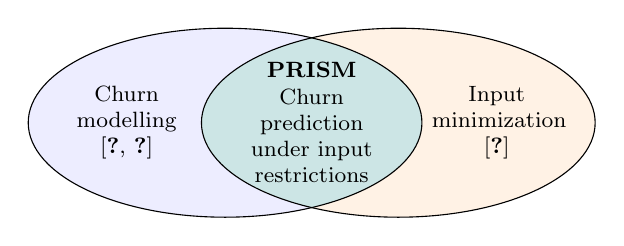
\begin{tikzpicture}[font=\footnotesize]
\fill[blue!7] (-1.1,0) ellipse (2.5 and 1.2);
\fill[orange!10] (1.1,0) ellipse (2.5 and 1.2);
\begin{scope}\clip (-1.1,0) ellipse (2.5 and 1.2);
\fill[teal!20] (1.1,0) ellipse (2.5 and 1.2);\end{scope}
\draw (-1.1,0) ellipse (2.5 and 1.2);\draw (1.1,0) ellipse (2.5 and 1.2);
\node[align=center,text width=1.65cm] at (-2.35,0) {Churn\\modelling\\\cite{mozer,neslin}};
\node[align=center,text width=1.65cm] at (2.35,0) {Input\\minimization\\\cite{goldsteen}};
\node[align=center,text width=2cm] at (0,0) {\textbf{PRISM}\\Churn prediction\\under input\\restrictions};
\end{tikzpicture}
\caption{Conceptual overlap of research aims. Placement illustrates this review's emphasis, not exclusive membership or an unstudied intersection.}
\Description{Two overlapping sets represent churn modelling and input minimization. PRISM is placed in their intersection.}\label{fig:venn}
\end{figure}

\section{Positioning PRISM}
PRISM studies how restricting customer information affects churn prediction. We propose three information tiers: basic administrative attributes; administrative and billing attributes; and all eligible account and service attributes. Each tier includes the information from the previous tier. We will check the dataset before assigning features to tiers and exclude identifiers and fields derived from the churn outcome. We will compare logistic regression and boosted trees, retraining each model for every tier. All experiments will use identical data splits and comparable tuning budgets, with preprocessing fitted only on training data.

We will report PR-AUC, ROC-AUC and churn recall, with uncertainty estimates. Recall will also be measured among a fixed proportion of customers ranked as most likely to leave. We will choose this proportion before evaluating the models. Feature counts will describe how much information each tier uses; they do not measure privacy protection. If the dataset has subscription details but no activity logs, our findings will apply only to restrictions on account information. Testing performance for new customers will require a separate evaluation of customers with short account histories. This benchmark will test how much predictive performance changes as more account information becomes available.

\bibliographystyle{ACM-Reference-Format}
\bibliography{bibliography}

\clearpage
\appendix
\section{AI-Assisted Editing Disclosure}

ChatGPT was used to improve clarity, grammar and readability,
reduce repetition, and simplify wording in the feature
selection, input minimization and project positioning
sections. It also assisted with LaTeX formatting.

\subsection{Original Unedited Student Draft}
Please refer to the original draft document submitted along with this document.
\end{document}
